\documentclass{article}
\usepackage{graphicx} % Required for inserting images
\usepackage{amsmath}
\usepackage{amssymb}
\usepackage{bm}
\usepackage{bbm}
\usepackage{color}
\usepackage{url}
\usepackage[export]{adjustbox}

\usepackage{braket}
\title{Quantum Paldus Transform}

\begin{document}
\section{Quantum Paldus Transformation as a gauging duality}
We can write the Quantum Paldus transform in terms of gauging maps using the language of tensor networks. First, we must gauge the global $U(1) \otimes SU(2)$ symmetry which will produce gauge fields labeled by irreps of $U(1)$ and $SU(2)$ with a boundary condition that transforms under $U(1) \otimes SU(2)$. This gauging map can be characterised by the following two tensors:
\begin{equation}
\centering
   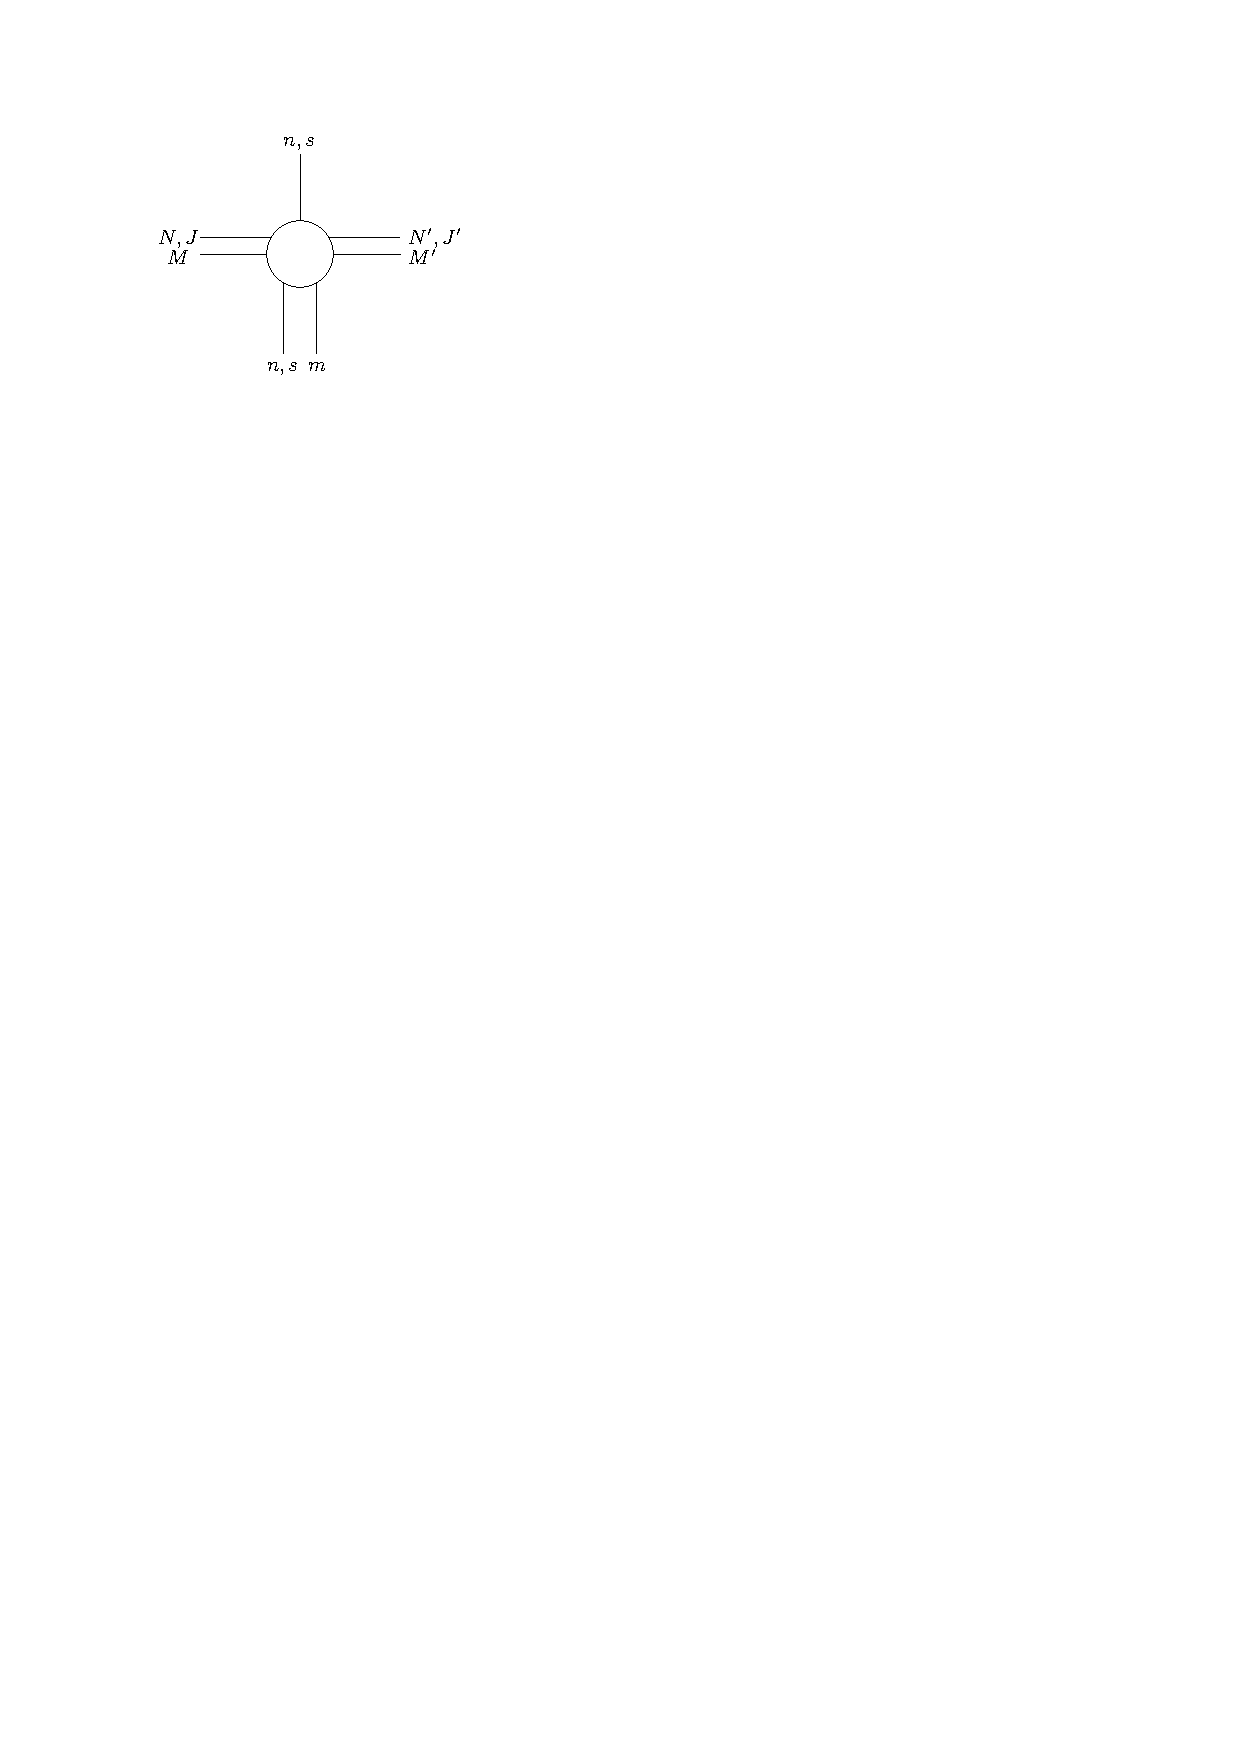
\includegraphics[scale=0.5,valign=c,page=1]{Quantum Paldus figs.pdf} = C_{J,M;s,m}^{J',M'} \delta_{N+n, N'}\ket{m}\ket{n,s}\bra{n,s}\otimes\ket{N,J}\bra{N',J'} \otimes\ket{M}\bra{M'}
\end{equation}
\begin{equation}
    \centering
   \includegraphics[scale=0.5,valign=c,page=2]{Quantum Paldus figs.pdf} =\ket{N,J}_L \bra{N,J}_R\bra{N,J}
\end{equation}
We combine this two tensors into the following gauging MPO:
\begin{equation}
    \centering
   \includegraphics[scale=0.5,valign=c,page=4]{Quantum Paldus figs.pdf}
\end{equation}

As we restrict the incoming values of $\ket{n,s}$ to $\ket{0,0}$, $\ket{1, \frac{1}{2}}$ and $\ket{2,0}$ the gauge fields can be used to disentangle the remaining matter degrees of freedom as $n = N'-N$ and $s = |J'-J|$. It would not be possible to disentangle the $s$ degree of freedom if larger values of $s$ were allowed.

Then we can apply a Kramers-Wannier-esk ungauging map to transform back to matter degrees of freedom with boundary conditions labeled by irreps of $U(1)$ and $SU(2)$. This gauging map is constructed of tensors of the following form:
\begin{equation}
   \centering
   \includegraphics[scale=0.5,valign=c,page=3]{Quantum Paldus figs.pdf} = \delta_{N'-N, \Delta N}\delta_{J'-J, \Delta J} \ket{N,J}_L \bra{N',J'}_R\bra{\Delta N,\Delta J}
\end{equation}
The combination of these MPOs gives us one MPO that performs the Quantum Paldus Transformation. 
\begin{equation}
    \centering
   \includegraphics[scale=0.5,valign=c,page=5]{Quantum Paldus figs.pdf}
\end{equation}
We can perform a local change of basis on the physical legs to move into an identical formulation as found in the original paper. The local change of basis are given by:
\begin{equation}
    \centering
   \includegraphics[scale=0.5,valign=c,page=9]{Quantum Paldus figs.pdf} =
       \begin{tabular}{|c|c|c|}
       \hline
           $\Delta N$ &$\Delta J$& $d$  \\ \hline
           0 & 0& 0 \\\hline
           1 & $\frac{1}{2}$& 1 \\\hline
           1 & $-\frac{1}{2}$& 2 \\\hline
           2 & 0& 3 \\\hline
       \end{tabular}
       \end{equation}
\begin{equation}
\label{eq:occupation_to_spins}
       \includegraphics[scale=0.5,valign=c,page=8]{Quantum Paldus figs.pdf}=
       \begin{tabular}{|c|c|c|c|}
       \hline
           $x_{\downarrow}x_{\uparrow}$ &$n$& $s$&$m$  \\ \hline
           00 & 0& 0&0 \\\hline
           01 & 1& $\frac{1}{2}$&$\frac{1}{2}$ \\\hline
           10 & 1& $\frac{1}{2}$&$-\frac{1}{2}$ \\\hline
           11 & 2& 0&0 \\\hline
       \end{tabular}
\end{equation}
and hence the Quantum Paldus Transformation is given by:
\begin{equation}
    \centering
   \includegraphics[scale=1,valign=c,page=6]{Quantum Paldus figs.pdf}
\end{equation}

We can use common techniques for converting MPOs into quantum circuits to convert this into a quantum circuit that implements the Quantum Paldus Transformation. First, we will need to pick the number of sites $\eta$ upon which we want the transform to act upon. This fixes the maximum values of $N$, $J$ and $M$ allowing us to truncate the bond dimension of the respective degrees of freedom and map these degrees of freedom to ancilla qubits. Then, we shift into the following form, and contract the tensors to find the unitary $U$:
\begin{equation}
    \centering
   \includegraphics[scale=1,valign=c,page=10]{Quantum Paldus figs.pdf} = \centering
   \includegraphics[scale=1,valign=c,page=11]{Quantum Paldus figs.pdf}
\end{equation}
We can then concatenate these unitaries together to form a quantum circuit for the full Quantum Paldus transformation:
\begin{equation}
    \centering
   \includegraphics[scale=0.5,valign=c,page=12]{Quantum Paldus figs.pdf} 
\end{equation}
Decomposing $U$ into a quantum circuit constructed of physically implementable gates is a non-trivial task.
\section{Generalised Quantum Paldus Transformation as a gauging duality}
In the previous section we restricted ourselves to acting upon two identical spinful fermionic modes which we could think of as an s orbital. We need not make this restriction, for example we could instead restrict to a p sub-shell which has six identical spinful fermionic modes with orbital angular momentum of 1.

If we utilise $jj$-coupling then the p sub-shell splits into two types of equivalent electrons with total angular momentum $\frac{3}{2}$ and $\frac{1}{2}$ respectively. Therefore, we can split the sub-shell into two sites with $4$ and $2$ fermionic modes each represented by a 6 particle Fock space with each mode corresponding to a different possible total angular momentum quantum number and main total angular momentum quantum number: $\ket{x_{\frac{3}{2}\frac{3}{2}}x_{\frac{3}{2}\frac{1}{2}}x_{\frac{3}{2}\frac{-1}{2}}x_{\frac{3}{2}\frac{-3}{2}}x_{\frac{1}{2}\frac{1}{2}}x_{\frac{1}{2}\frac{-1}{2}}}$. It is trivial to map from this Fock space to qubits using the Jordan-Wigner mapping. Therefore, the first step of our generalisation is to find an equivalent basis transformation to \eqref{eq:occupation_to_spins} from occupation basis to spin basis. An important distinction to \eqref{eq:occupation_to_spins} is that here each occupation basis element maps to multiple possible spin states due to the fusion of the spin and orbital angular momentum. Therefore, in order to distinguish these multiplicities we require an additional quantum number, we have chosen to use the number of particles in the $\frac{1}{2}$ subset of fermonic modes $i$.

% Best reference for jj coupling \cite{gauerke1994simple}.

   \begin{tabular}{|c|c|c|c|c|}
   \hline
       $x_{\frac{3}{2}\frac{3}{2}}x_{\frac{3}{2}\frac{1}{2}}x_{\frac{3}{2}\frac{-1}{2}}x_{\frac{3}{2}\frac{-3}{2}}x_{\frac{1}{2}\frac{1}{2}}x_{\frac{1}{2}\frac{-1}{2}}$ &$n$& $s$&$m$&$i$  \\ \hline
       000000 & 0& 0&0&0 \\\hline
       100000 & 1& $\frac{3}{2}$&$\frac{3}{2}$&0 \\\hline
       010000 & 1& $\frac{3}{2}$&$\frac{1}{2}$&0 \\\hline
       001000 & 1& $\frac{3}{2}$&$-\frac{1}{2}$&0 \\\hline
       000100 & 1& $\frac{3}{2}$&$-\frac{3}{2}$&0 \\\hline
       000010 & 1& $\frac{1}{2}$&$\frac{1}{2}$&1 \\\hline
       000001 & 1& $\frac{1}{2}$&$-\frac{1}{2}$&1 \\\hline
       110000 & 2&$2$ &$2$&0 \\\hline
       101000 & 2&$2$ &$1$&0 \\\hline
       100100 & 2&$2$ &$0$&0 \\\hline
       100010 & 2&$2$ &$2$&1 \\\hline
       100001 & 2&$2$ &$1$&1 \\\hline
       011000 & 2&$0$ &$0$&0 \\\hline
       010100 & 2&$2$ &$-1$&0 \\\hline
       010010 & 2& $1$&$1$&1 \\\hline
       010001 & 2&$2$ &$0$&1 \\\hline
       001100 & 2&$2$ &$-2$&0 \\\hline
       001010 & 2&$1$ &$0$&1 \\\hline
       001001 & 2&$2$ &$-1$&1 \\\hline
       000110 & 2&$1$ &$-1$&1 \\\hline
       000101 & 2&$2$ &$-2$&1 \\\hline
       000011 & 2&$0$ &$0$&2 \\\hline
       111000 & 3& $\frac{3}{2}$&$\frac{3}{2}$&0 \\\hline
       110100 & 3&$\frac{3}{2}$ &$\frac{1}{2}$&0 \\\hline 
       110010 & 3&$\frac{5}{2}$ &$\frac{5}{2}$&1 \\\hline 
       110001 & 3& $\frac{5}{2}$&$\frac{3}{2}$&1 \\\hline 
       101100 & 3&$\frac{3}{2}$ &$-\frac{1}{2}$&0 \\\hline
       101010 & 3&$\frac{3}{2}$ &$\frac{3}{2}$&1 \\\hline
       101001 & 3& $\frac{1}{2}$&$-\frac{1}{2}$&1 \\\hline
       100110 & 3&$\frac{5}{2}$ &$\frac{1}{2}$&1 \\\hline
       100101 & 3& $\frac{5}{2}$&$-\frac{1}{2}$&1 \\\hline       
       100011 & 3&$\frac{3}{2}$ &$\frac{3}{2}$&2 \\\hline 
       011100 & 3& $\frac{3}{2}$&$-\frac{3}{2}$&0 \\\hline
       011010 & 3&$\frac{3}{2}$ &$\frac{1}{2}$&1 \\\hline
       011001 & 3&$\frac{3}{2}$ &$-\frac{1}{2}$&1 \\\hline
       010110 & 3&$\frac{1}{2}$ &$-\frac{1}{2}$&1 \\\hline
       010101 & 3&$\frac{5}{2}$ &$-\frac{3}{2}$&1 \\\hline
       010011 & 3& $\frac{3}{2}$&$\frac{1}{2}$&2 \\\hline
       001110 & 3&$\frac{3}{2}$ &$-\frac{3}{2}$&1 \\\hline
       001101 & 3&$\frac{5}{2}$ &$-\frac{5}{2}$&1 \\\hline
       001011 & 3& $\frac{3}{2}$&$-\frac{1}{2}$&2 \\\hline
       000111 & 3& $\frac{3}{2}$&$-\frac{3}{2}$&2 \\\hline
   \end{tabular}
   \begin{tabular}{|c|c|c|c|c|}
   \hline
       $x_{\frac{3}{2}\frac{3}{2}}x_{\frac{3}{2}\frac{1}{2}}x_{\frac{3}{2}\frac{-1}{2}}x_{\frac{3}{2}\frac{-3}{2}}x_{\frac{1}{2}\frac{1}{2}}x_{\frac{1}{2}\frac{-1}{2}}$ &$n$& $s$&$m$&$i$  \\ \hline
       111100 & 4& 0&0&0 \\\hline
       111010 & 4&2 &2&1 \\\hline
       111001 & 4& 1&1&1 \\\hline
       110110 & 4&2 &1&1 \\\hline
       110101 & 4&2 &0&1 \\\hline
       110011 & 4& 2&2&2 \\\hline
       101110 & 4& 1&0&1 \\\hline
       101101 & 4&2 &-1&1 \\\hline
       101011 & 4& 2&1&2 \\\hline
       100111 & 4&2 &0&2 \\\hline
       011110 & 4&1 &-1&1 \\\hline
       011101 & 4& 2&-2&1 \\\hline
       011011 & 4& 0&0&2 \\\hline
       010111 & 4& 2&-1&2 \\\hline
       001111 & 4&2 &-2&2 \\\hline
       111110 & 5&$\frac{1}{2}$ &$\frac{1}{2}$&1 \\\hline
       111101 & 5&$\frac{1}{2}$ &$-\frac{1}{2}$&1 \\\hline
       111011 & 5&$\frac{3}{2}$ &$\frac{3}{2}$&2 \\\hline
       110111 & 5&$\frac{3}{2}$ &$\frac{1}{2}$&2 \\\hline
       101111 & 5&$\frac{3}{2}$ &$-\frac{1}{2}$&2 \\\hline
       011111 & 5& $\frac{3}{2}$&$-\frac{3}{2}$&2 \\\hline
       111111 & 6&0 &0&2 \\\hline
   \end{tabular}

It is possible to map from the more common $LS$-coupling basis $x_{1\uparrow}x_{1\downarrow}x_{0\uparrow}x_{0\downarrow}x_{-1\uparrow}x_{-1\downarrow}$ to the $jj$-coupling basis by performing Clebsch-Gordan coupling. For example:
\begin{equation}
    \ket{110000}_{LS} = C_{1,1;\frac{1}{2},-\frac{1}{2}}^{\frac{3}{2},\frac{1}{2}}\ket{110000}_{jj} + C_{1,1;\frac{1}{2},-\frac{1}{2}}^{\frac{1}{2},\frac{1}{2}}\ket{100010}_{jj}
\end{equation}
\begin{multline}
    \ket{011000}_{LS} = C_{1,0;\frac{1}{2},\frac{1}{2}}^{\frac{3}{2},-\frac{1}{2}}C_{1,1;\frac{1}{2},-\frac{1}{2}}^{\frac{3}{2},\frac{1}{2}}\ket{011000}_{jj} + C_{1,0;\frac{1}{2},\frac{1}{2}}^{\frac{3}{2},-\frac{1}{2}}C_{1,1;\frac{1}{2},-\frac{1}{2}}^{\frac{1}{2},\frac{1}{2}}\ket{001010}_{jj} +\\ C_{1,0;\frac{1}{2},\frac{1}{2}}^{\frac{1}{2},-\frac{1}{2}}C_{1,1;\frac{1}{2},-\frac{1}{2}}^{\frac{3}{2},\frac{1}{2}}\ket{010001}_{jj}+ C_{1,0;\frac{1}{2},\frac{1}{2}}^{\frac{1}{2},-\frac{1}{2}}C_{1,1;\frac{1}{2},-\frac{1}{2}}^{\frac{1}{2},\frac{1}{2}}\ket{000011}_{jj}
\end{multline}

If we take the values of $n,s,m$ from the previous table as the non-zero input values of the MPO tensor, then we can no longer simply disentangle the $s$ matter degree of freedom after applying the tensor. Therefore, after we perform the ungauging map to get $\Delta N$ and $\Delta J$, we have $\Delta N$, $\Delta J$, $s$ and $i$ as our new onsite Hilbert space. We can consider all of the possible values for these to construct a local basis $d$:

       \begin{tabular}{|c|c|c|c|c|}
       \hline
           $\Delta N$ &$\Delta J$& $s$ &$i$&$d$ \\ \hline
           0 & 0& 0&0&0 \\\hline
           1 & $\frac{3}{2}$& $\frac{3}{2}$&0&1 \\\hline
           1 & $\frac{1}{2}$& $\frac{3}{2}$&0&2 \\\hline
           1 & $-\frac{1}{2}$& $\frac{3}{2}$&0&3 \\\hline
           1 & $-\frac{3}{2}$& $\frac{3}{2}$&0&4 \\\hline           
           1 & $\frac{1}{2}$& $\frac{1}{2}$&1&5 \\\hline               
           1 & $-\frac{1}{2}$& $\frac{1}{2}$&1&6 \\\hline            
           2 & $2$& $2$&0&7 \\\hline            
           2 & $1$& $2$&0&8 \\\hline            
           2 & $0$& $2$&0&9 \\\hline            
           2 & $-1$& $2$&0&10 \\\hline            
           2 & $-2$& $2$&0&11 \\\hline            
           2 & $2$& $2$&1&12 \\\hline            
           2 & $1$& $2$&1&13 \\\hline            
           2 & $0$& $2$&1&14 \\\hline            
           2 & $-1$& $2$&1&15 \\\hline            
           2 & $-2$& $2$&1&16 \\\hline           
           2 & $1$& $1$&1&17 \\\hline         
           2 & $0$& $1$&1&18 \\\hline         
           2 & $-1$& $1$&1&19 \\\hline         
           2 & $0$& $0$&0&20 \\\hline        
           2 & $0$& $0$&2&21 \\\hline        
           3 & $\frac{5}{2}$& $\frac{5}{2}$&1&22 \\\hline       
           3 & $\frac{3}{2}$& $\frac{5}{2}$&1&23 \\\hline       
           3 & $\frac{1}{2}$& $\frac{5}{2}$&1&24 \\\hline       
           3 & $-\frac{1}{2}$& $\frac{5}{2}$&1&25 \\\hline       
           3 & $-\frac{3}{2}$& $\frac{5}{2}$&1&26 \\\hline       
           3 & $-\frac{5}{2}$& $\frac{5}{2}$&1&27 \\\hline       
           3 & $\frac{3}{2}$& $\frac{3}{2}$&0&28\\\hline       
           3 & $\frac{1}{2}$& $\frac{3}{2}$&0&29 \\\hline       
           3 & $-\frac{1}{2}$& $\frac{3}{2}$&0&30 \\\hline       
           3 & $-\frac{3}{2}$& $\frac{3}{2}$&0&31 \\\hline
           3 & $\frac{3}{2}$& $\frac{3}{2}$&1&32 \\\hline       
           3 & $\frac{1}{2}$& $\frac{3}{2}$&1&33 \\\hline       
           3 & $-\frac{1}{2}$& $\frac{3}{2}$&1&34 \\\hline       
           3 & $-\frac{3}{2}$& $\frac{3}{2}$&1&35 \\\hline
           3 & $\frac{3}{2}$& $\frac{3}{2}$&2&36 \\\hline       
           3 & $\frac{1}{2}$& $\frac{3}{2}$&2&37 \\\hline       
           3 & $-\frac{1}{2}$& $\frac{3}{2}$&2&38 \\\hline       
           3 & $-\frac{3}{2}$& $\frac{3}{2}$&2&39 \\\hline       
           3 & $\frac{1}{2}$& $\frac{1}{2}$&1&40 \\\hline
           3 & $-\frac{1}{2}$& $\frac{1}{2}$&1&41 \\\hline       
       \end{tabular}
       \begin{tabular}{|c|c|c|c|c|}
       \hline
           $\Delta N$ &$\Delta J$& $s$ &$i$&$d$ \\ \hline         
           4 & $2$& $2$&2&42 \\\hline            
           4 & $1$& $2$&2&43 \\\hline            
           4 & $0$& $2$&2&44 \\\hline            
           4 & $-1$& $2$&2&45 \\\hline            
           4 & $-2$& $2$&2&46 \\\hline            
           4 & $2$& $2$&1&47 \\\hline            
           4 & $1$& $2$&1&48 \\\hline            
           4 & $0$& $2$&1&49 \\\hline            
           4 & $-1$& $2$&1&50 \\\hline            
           4 & $-2$& $2$&1&51 \\\hline           
           4 & $1$& $1$&1&52 \\\hline         
           4 & $0$& $1$&1&53 \\\hline         
           4 & $-1$& $1$&1&54 \\\hline         
           4 & $0$& $0$&0&55 \\\hline        
           4 & $0$& $0$&2&56 \\\hline     
           5 & $\frac{3}{2}$& $\frac{3}{2}$&2&57 \\\hline
           5 & $\frac{1}{2}$& $\frac{3}{2}$&2&58 \\\hline
           5 & $-\frac{1}{2}$& $\frac{3}{2}$&2&59 \\\hline
           5 & $-\frac{3}{2}$& $\frac{3}{2}$&2&60 \\\hline           
           5 & $\frac{1}{2}$& $\frac{1}{2}$&1&61 \\\hline               
           5 & $-\frac{1}{2}$& $\frac{1}{2}$&1&62 \\\hline   
           6 & 0& 0&2&63 \\\hline
       \end{tabular}

% The $p$-subshell contains 6 electrons. If all the electrons within the orbital are treated identically by the Hamiltonian than we have an $U(1) \times SU(6)$ symmetry. In reality this symmetry is not achieved as the $p$-subshell is constructed of 3 orbitals, and the Hamiltonian contains differing interactions between the electrons depending upon which orbital they lie in and what intrinsic spin they have. These terms break the symmetry in different ways. The orbit-orbit interactions and spin-spin interactions break the $U(1) \times SU(6)$ down to subgroup $U(1) \times SO(3) \times SU(2)$. The spin-orbit interactions break the $U(1) \times SU(6)$ down to subgroup $U(1) \times SU(2)$. In the previous section we consider this regime with spin-orbit interactions such that the electrons spin and orbital angular momentum couple to each other. If we instead consider Hamiltonians with no spin-orbit interactions then the symmetry is given by $U(1) \times SO(3) \times SU(2)$ and we can further modify the Quantum Paldus Transformation to take advantage of this increased symmetry.

We can instead utilise the LS-coupling to write the $p$ sub-shell as a 6 particle Fock space with each mode corresponding to a combination of possible spin and orbital angular momentum: $\ket{x_{1\uparrow}x_{1\downarrow}x_{0\uparrow}x_{0\downarrow}x_{-1\uparrow}x_{-1\downarrow}}$. Again the first step in producing the Quantum Paldus Transform is to find the basis transformation from this occupation basis to the spin basis. As we now have a $U(1) \times SO(3)\times SU(2)$ symmetry we no longer have any mutliplicities to worry about, and instead get two sets of spin irrep labels and values $s$, $m_s$ and $l$, $m_l$:
   \begin{tabular}{|c|c|c|c|c|c|}
   \hline
       $\ket{x_{1\uparrow}x_{1\downarrow}x_{0\uparrow}x_{0\downarrow}x_{-1\uparrow}x_{-1\downarrow}}$ &$n$& $s$&$m_s$&$l$&$m_l$  \\ \hline
       000000 & 0& 0&0&0&0 \\\hline
       100000 & 1&$\frac{1}{2}$ &$\frac{1}{2}$&1&1 \\\hline
       010000 & 1&$\frac{1}{2}$ &$-\frac{1}{2}$&1&1 \\\hline
       001000 & 1&$\frac{1}{2}$ &$\frac{1}{2}$&1&0 \\\hline
       000100 & 1&$\frac{1}{2}$ &$-\frac{1}{2}$&1&0 \\\hline
       000010 & 1&$\frac{1}{2}$ &$\frac{1}{2}$&1&-1 \\\hline
       000001 & 1&$\frac{1}{2}$ &$-\frac{1}{2}$&1&-1 \\\hline
       110000 & 2& 0&0&2 &2  \\\hline
       101000 & 2& 1&1&1 &1  \\\hline
       100100 & 2& 0&0&2 &1  \\\hline
       100010 & 2& 1&1&1 &0  \\\hline
       100001 & 2& 0&0&2&0  \\\hline
       011000 & 2& 1&0&1 &1  \\\hline
       010100 & 2& 1&-1&1 &1  \\\hline
       010010 & 2& 1&0&1 &0  \\\hline
       010001 & 2& 1&-1&1 &0  \\\hline
       001100 & 2& 0&0&0 &0  \\\hline
       001010 & 2& 1&1&1 &-1  \\\hline
       001001 & 2& 0&0&2 &-1  \\\hline
       000110 & 2& 1&0&1 &-1  \\\hline
       000101 & 2&1 &-1&1 &-1  \\\hline
       000011 & 2& 0&0&2 &-2  \\\hline
       
       
       \end{tabular}
       
We then apply the quantum paldus transformation separately to the labels $n,s,m_s$ and $n,l,m_l$. We again apply the ungauging map to get $\Delta N,\Delta J_s$ and $\Delta N, \Delta J_l$, obviously one of the duplicate $\Delta N$ can be disentangled along with the remaining $n$ label. We cannot disentangle the $s$ and $l$ so they must be included in local basis $d$ we construct:

       \begin{tabular}{|c|c|c|c|c|c|}
       \hline
           $\Delta N$ &$\Delta J_s$& $s$ &$\Delta J_l$&$l$&$d$ \\ \hline
           0 & 0& 0&0&0&0 \\\hline
           1 & $\frac{1}{2}$& $\frac{1}{2}$&1&1&1 \\\hline
           1 & $-\frac{1}{2}$& $\frac{1}{2}$&1&1&2 \\\hline
           1 & $\frac{1}{2}$& $\frac{1}{2}$&0&1&3 \\\hline
           1 & $-\frac{1}{2}$& $\frac{1}{2}$&0&1&4 \\\hline
           1 & $\frac{1}{2}$& $\frac{1}{2}$&-1&1&5 \\\hline
           1 & $-\frac{1}{2}$& $\frac{1}{2}$&-1&1&6 \\\hline
           2 & $0$& $0$&2&2&7 \\\hline
           2 & $0$& $0$&1&2&8 \\\hline
           2 & $0$& $0$&0&2&9 \\\hline
           2 & $0$& $0$&-1&2&10 \\\hline
           2 & $0$& $0$&-2&2&11 \\\hline
           2 & 1& $1$&1&1&12 \\\hline
           2 & 1& $1$&0&1&13 \\\hline
           2 & 1& $1$&-1&1&14 \\\hline
           2 & 0& $1$&1&1&15 \\\hline
           2 & 0& $1$&0&1&16 \\\hline
           2 & 0& $1$&-1&1&17 \\\hline
           2 & -1& $1$&1&1&18 \\\hline
           2 & -1& $1$&0&1&19 \\\hline
           2 & -1& $1$&-1&1&20 \\\hline
           2 & 0& 0&0&0&21 \\\hline
           
           \end{tabular}


In principle, the orbit-orbit interactions and and spin-spin interactions could break down the $U(1) \times SO(3) \times SU(2)$ into subgroup $U(1) \times H \times SU(2)$ where $H$ is some subgroup of $SO(3)$, this would allow us to expand the Quantum Paldus transformation to encompass shells with arbitary point group symmetry (look here for more info \url{https://en.m.wikipedia.org/wiki/Configuration_state_function}). We could also consider the case with spin-orbit coupling in which case the symmetry would break down to a the double group of the point group symmetry: $U(1) \times H_D$. In both of these examples we should be able to replicate the gauging map from before but now instead with finite groups.



% Is this statement correct. In the second shell of a hydrogen atom there are 8 possible electronic modes, these can be labelled by quantum numbers n, l, m_l and m_s. For 2 of them they have n,l = 2,0 and for 6 of them they have n,l = 2, 1. If your hamiltonian that you apply has no dependance on the m_l or m_s value of the angular momentum or ths, then you can say your hamiltonian has SO(3)xSU(2) symetry and the 2 electrons in the s subshell are equivalent and the 6 in the p subshell are equivalent. If your hamiltonian has any dependance on the m_l value of these electrons you lose the SO(3) symmetry for the p subshell and now the 2 electrons in the s subshell are still equivalent but the p subshell splits into 3 separate orbitals with differing m_l values (the electrons in each orbital are still equivalent). Similarly if you have some sort of coupling between the total spin and the total orbital angular momentum in your hamiltonian but no other dependance on the m_l or m_s value, then the energy depends on the sum of $j=s+l$, so you split the p subshell into 2 different orbitals, now you have a s subshell with 2 equivalent electrons, one orbital with 4 equivalent electrons with $m_j = -3/2,-1/2,1/2,3/2$ and one orbital with 2 equivalent electrons. If you have dependance on m_l and spin-orbit interactions then the subshell still remains the same with 2 equivalent electrons, but the p subshell now splits into 6 different non-equivalent types of electronic modes. Bonding between two atoms is just dependant on the columb interaction so is independant of the spin, hence if we have no spin-orbit interactions we retain the $SU(2)$ symmetry but we break the local $SO(3)$ symmetry entirely. In the new many body larger space there may be a new point group symmetry of the molecule but it is not built out of a local symmetry. However, for a lattice this is different, the point group symmetry of the lattice reduces to a local rotational symmetry, therefore we can split the atomic orbitals into irreps of the point group and orbitals in the same irrep are equivalent.
% \pagebreak

% Name for the coupling of successive L-S coupled shells is parental history, and it does proceed how one would imagine by first coupling all the Ls and Ss separately. \url{https://www.sternwarte.uni-erlangen.de/docs/theses/2012-10_Laska.pdf}

% \section{Existing Quantum Paldus Transformation}
% The Quantum Paldus transform can be expressed as an MPO intertwiner between dual models. The transformation takes a spin-free particle conserving fermionic Hamiltonian to a Hamiltonian with no global symmetry acting upon a Hilbert space associated with a particular particle number and total spin. Therefore, we must construct an MPO duality that transforms the categorical symmetry $\mathcal{C}=\text{Rep}(U(1)) \boxtimes \text{Rep}(SU(2))$ to Vec $\boxtimes$ Vec. $\text{Rep}(U(1))$ corresponds to the number symmetry. The simple objects of this fusion category look like tuples of simple objects from $\text{Rep}(U(1))$ and $\text{Rep}(SU(2))$.

% Given any symmetry category $\mathcal{C}$ we may pick any module category $\mathcal{M}$ of this symmetry, and then find an input category $\mathcal{D}$ such that $\mathcal{M}$ is a bi-module category of $\mathcal{C}$ and $\mathcal{D}$. The easiest choice of $\mathcal{M}$ is Vec $\boxtimes$ Vec, which corresponds to the input category $\mathcal{D} = \mathcal{C} = \text{Rep}(U(1)) \boxtimes \text{Rep}(SU(2))$. {\color{blue} If we pick $\mathcal{M} = sVec /<\psi = \mathbbm{1}>$ will this still give $\mathcal{D} = \mathcal{C}$, presumably it will mean $\mathcal{X} = \beta$}

% Now we have chosen an input category we are free to choose a new module category $\mathcal{N}$ of $\mathcal{D}$, which we can use to construct a new Hamiltonian with new symmetry $\mathcal{C}'$. We wish our new symmetry to be $\mathcal{C}'=$Vec $\boxtimes$ Vec, so we should choose $\mathcal{N} = \mathcal{D} = \mathcal{C} = \text{\text{Rep}(U(1)) \boxtimes \text{Rep}(SU(2))$.

% As we wish to construct an MPO intertwinner we must go one step further and consider the possible module functors $\mathcal{X}$ between $\mathcal{M}$ and $\mathcal{N}$ over $\mathcal{D}$. Fortunately for our choices we have $\mathcal{X} = Fun_{\mathcal{D}}(\mathcal{M}, \mathcal{N}) = Fun_{\text{Rep}(U(1)) \boxtimes \text{Rep}(SU(2))}(\text{Vec $\boxtimes$ Vec},\text{Rep}(U(1)) \boxtimes \text{Rep}(SU(2))) = \text{Vec}$.

% We now have enough information to write down the MPO intertwinner:
% \begin{figure}[htbp]
%     \centering
%     % \includegraphics[width=0.5\linewidth]{}
%     \caption{Caption}
%     \label{fig:placeholder}
% \end{figure}

% This can be rewritten as the following tensor from $(n_i, S_i, m)$ to $(M,N_{i-\frac{1}{2}},S_{i-\frac{1}{2}},N_{i+\frac{1}{2}},S_{i+\frac{1}{2}},M')$:
% \begin{figure}[htbp]
%     \centering
%     % \includegraphics[width=0.5\linewidth]{}
%     \caption{Caption}
%     \label{fig:placeholder}
% \end{figure}


% To transform this MPO intertwiner into the Quantum Paldus transformation we must compose it with a Kramers-Wannier like duality which maps the $n_{i-\frac{1}{2}}, S_{i-\frac{1}{2}}$ values to $\Delta N_{i}, \Delta S_i$ with the total particle number $N$ and total spin $S$ appearing as boundary conditions.

% \begin{figure}[htbp]
%     \centering
%     % \includegraphics[width=0.5\linewidth]{}
%     \caption{Caption}
%     \label{fig:placeholder}
% \end{figure}

% We restrict the initial Hilbert space to two indistinguishable spinful fermions per site, and hence our onsite Hilbert space is given by $0 \oplus \frac{1}{2} \oplus 0$. Therefore, we pick $\{\alpha\} = {(0,0), (1,\frac{1}{2}), (2,0)}$. Hence the only possible values of $(n_{i}, s_i,m_i)$ are $(0,0,0)$, $(1, \frac{1}{2},\frac{1}{2})$,$(1, \frac{1}{2},-\frac{1}{2})$ and $(2,0,0)$, and the only possible values of $(\Delta N_{i}, \Delta S_i)$ are $(0,0)$, $(1,\frac{1}{2})$,$(1,-\frac{1}{2})$ and $(2,0)$ which are in direct correspondence with the $\bm d$ step vectors in the Quantum Paldus transform.

% \section{Generalised Quantum Paldus Transformation}
% In the existing Quantum Paldus Transformation we restricted the onsite Hilbert space to be that of an 1s orbital. We can relax this and consider a generalised Quantum Paldus transformation that acts upon arbitrary electronic configurations. This is easily achieved by using the same MPO interwiner as before, but instead of restricting to the Hilbert space of the 1s orbital we restrict to the Hilbert space of the desired orbital. 

% To accomplish this we consider all the possible number of particles $N_i$ that could be in the orbital. We then utilise the $j-j$ coupling scheme whereby each electrons spin $S$ and orbital angular momentum $L$ are first coupled to give a $(1,j)$ per electron ($j = L \pm \frac{1}{2}$). Then all of these $(1,j)$s are coupled to give a direct sum of levels $(N_i,S_i)$. Only the couplings that obey the pauli exclusion principle are allowed. For each possible level $(N_i,S_i)$ we include $(N_i,S_i)$ in $\{\alpha\}$. Different micro-states may produce the same levels (e.g. $\frac{3}{2} \otimes\frac{1}{2} = 2 \oplus 1$ and $\frac{3}{2} \otimes\frac{3}{2} = 2 \oplus 0$) but this is not a problem we simply have to include multiple copies of the same object in $\{\alpha\}$.



% % The transformation acts upon spin-free fermionic Hamiltonians which can be written in terms of ladder operators:
% % \begin{equation}
% %     E_{ij} = \sum_{\mu} a^{\dagger}_{i \mu}a_{j \mu} \>\>\>\>\> \mathcal{E}_{\mu \nu} = \sum_i a^{\dagger}_{i \mu} a_{i \nu}
% % \end{equation}
% % for $i \in \{1, \dots, d\}$ and $\mu = \pm \frac{1}{2}$. These operators obey the following commutation relations:
% % \begin{equation}
% %     [E_{ij}, E_{kl}] = \delta_{jk}E_{il} - \delta_{il}E_{jk}  \>\>\>\>\> [\mathcal{E}_{\mu \nu}, \mathcal{E}_{\sigma \tau}] = \delta_{\nu \sigma}\mathcal{E}_{\mu \tau} - \delta_{\mu \tau}\mathcal{E}_{\sigma \nu}\>\>\>\>\> [E_{ij}, E_{\mu \nu}] = 0
% % \end{equation}
% % These commutation relations imply  $E_{ij}$ and $\mathcal{E}_{\mu \nu}$ are representations of the Lie algebras $\mathfrak{gl}(d)$ and $\mathfrak{gl}(2)$ respectively. 


% % is given by the module functor from module category $\mathcal{M} = \text{Vec} \boxtimes \text{Vec}$ to $\mathcal{N} = \text{Rep}(U(1)) \boxtimes \text{Rep}(SU(2))$ over input category $\mathcal{D} = \text{Rep}(U(1)) \boxtimes \text{Rep}(SU(2))$. 
% The Schur transform maps from $(\mathbb{C}^d)^{\otimes n}$ to $\oplus_{\lamba} V_{\lambda} \otimes P_{\lambda}$ where $V_{\lambda}$ are irreps of $U(d)$ and $P_{\lambda}$ are irreps of $S_n$.

% If we consider what happens to any element $\pi$ of $S_n$ under this transformation it is mapped to $\sum_{\lambda} \ket{\lambda}\bra{\lambda}\otimes \mathbb{I} \otimes P_{\lambda}(\pi)$. Therefore, it will commute with any unitary that acts solely on the first register (e.g. $V = \mathbb{I} \otimes \tilde V \otimes \mathbb{I}$). Hence, I was wondering is it true that I can generate an equivariant circuit by conjugating $V$ with the Schur transform $U_{sch}$. That is to say is the following equation true:
% $$
% [U_{sch}^{\dagger} (\mathbb{I} \otimes \tilde V \otimes \mathbb{I}) U_{sch}, \pi] = 0 \forall \pi \in S_n
% $$ 

% I know that the equivariant circuit $U^{\otimes n}$ goes to $\sum_{\lambda} \ket{\lambda}\bra{\lambda}\otimes V_{\lambda}(U) \otimes \mathbb{I}$, so maybe the equivariant circuit I generate above can be decomposed into this tensor product form in which case it is no use.
\end{document}
